\section{Design \& Methods}

The DeepDuct model begins with a so-called ``off-the-shelf'' ConvNet architecture; namely the VGG16 model pre-trained on the general-purpose ImageNet dataset \citep{simonyan2014,deng2009,imagenet}. The pre-trained VGG16 model was fine-tuned on the BreakHis dataset, a dataset comprised of approximately 8,000 images of H\&E stained human mammary biopsy sections classified according to World Health Organisation (WHO) guidelines \citep{spanhol2016, who_breast}. Abbreviations for the class names present in the BreakHis dataset are used throughout this manuscript, and within the model itself. Refer to Appendix A for a legend of these class codes. \par

The VGG16 model was implemented with Keras using TensorFlow as the back-end \citep{chollet2015, tensorflow}. A Keras/TensorFlow implementation of Grad-CAM implemented in the Keras-Vis library was used to generate attention maps from the BreakHis-trained VGG16 model \citep{raghakot}.\par

Plots created with the matplotlib and searborn libraries \citep{hunter2007, seaborn}.

\begin{figure}[h]
	\begin{center}
		\caption{Examples from the ImageNet and BreakHis Datasets \label{fig:imagenet_v_breakhis}}
	\end{center}
	\includegraphics[width=160mm]{figures/deepduct/imagenet_v_breakhis.pdf}
	\begin{singlespace}
		\textit{Legend} --- Thumbnails from some selected classes of the (a) ImageNet and (b) BreakHis datasets. The DeepDuct model makes use of a ConvNet model pre-trained on the ImageNet dataset and repurposed for classifying images according to the BreakHis dataset via transfer learning. The ImageNet ILSVRC2014 dataset is comprised of $\approx150,000$ images belonging to 1,000 classes, and the BreakHis dataset is comprised of 8,000 images belonging to 8 classes. 
	\end{singlespace}
	
\end{figure}

\begin{figure}[h]
	\begin{center}
		\caption{Schematic of the VGG16 ConvNet Architecture and its Fine-Tuning \label{fig:vgg_arch}}
	\end{center}
	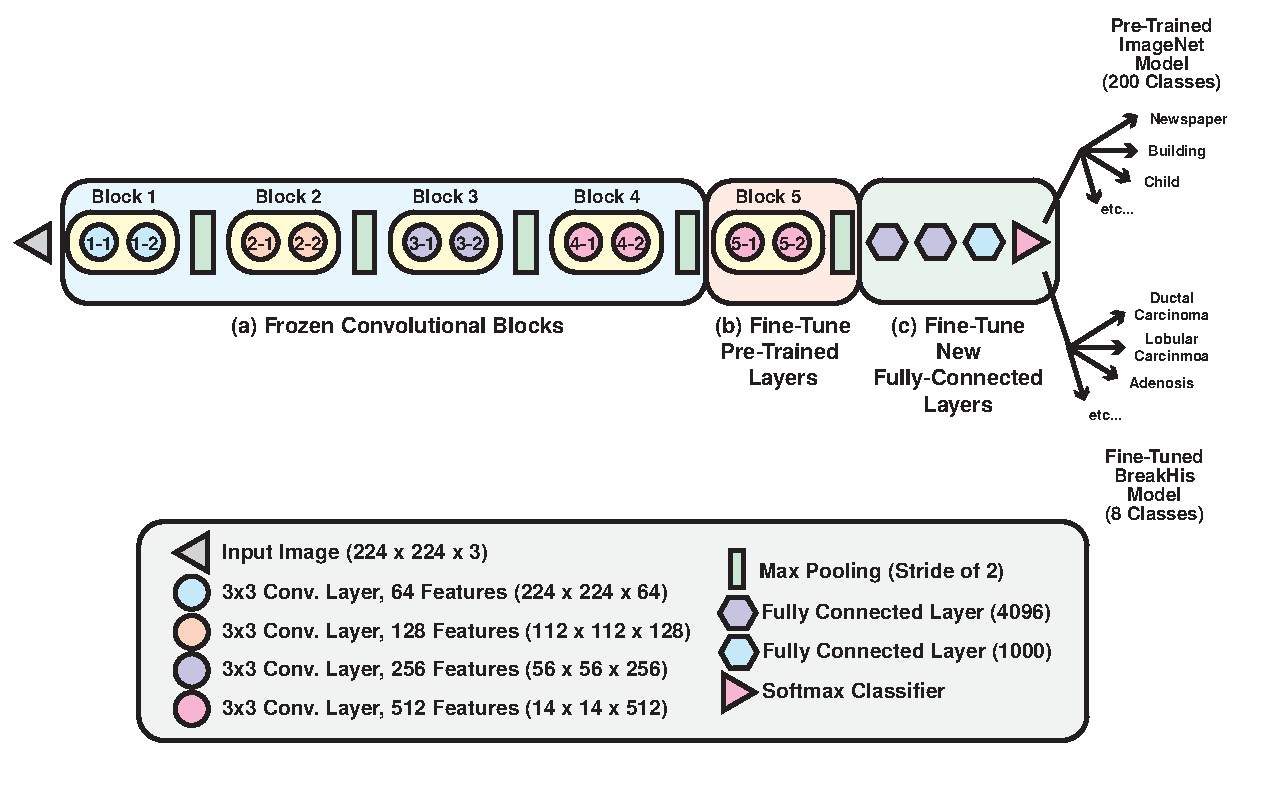
\includegraphics[width=160mm]{figures/deepduct/vgg_overview.pdf}
	\begin{singlespace}
		\textit{Legend} --- The VGG16 model is comprised of 16 weight layers, making up five convolutional blocks and a fully-connected classifier. Fine-tuning a pre-trained VGG16 model involves freezing the first four blocks (a), continuing to train the fifth block (b) against the new dataset (in this case, BreakHis) through backpropagation, and finally training a new fully-connected classifier against the new dataset (c).
	\end{singlespace}
	
\end{figure}